\documentclass[10pt]{article}
\usepackage[paperwidth=11.8cm,paperheight=4.5cm,margin=0pt]{geometry}
\usepackage{amsmath,amssymb}
\usepackage{mathptmx}
\renewcommand{\hbar}{\mathchar'26\mkern-9mu h}
\usepackage{tikz}
\pagestyle{empty}
\begin{document}
\special{papersize=11.8cm,4.5cm}
\noindent
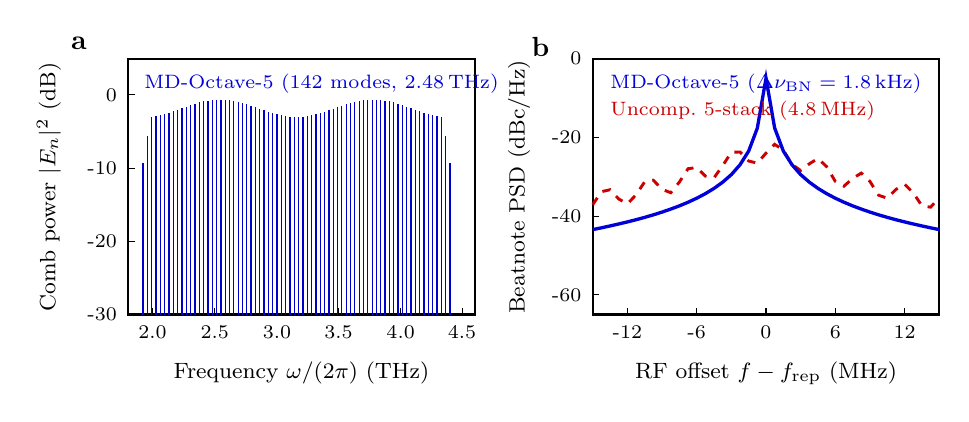
\begin{tikzpicture}[x=1cm,y=1cm,font=\footnotesize]
  % Panel a: Octave-spanning FM comb spectrum (1.92 - 4.40 THz)
  \node[anchor=north west,font=\bfseries\normalsize] at (0.10,4.35) {a};
  \draw[thick] (0.95,0.70) rectangle (5.35,3.95);
  \foreach \v/\y in {-30/0.70, -20/1.63, -10/2.56, 0/3.49} {
    \draw (0.95,\y) -- (1.03,\y);
    \node[left,font=\scriptsize] at (0.93,\y) {\v};
  }
  \foreach \fval/\xpos in {2.0/1.26, 2.5/2.05, 3.0/2.84, 3.5/3.62, 4.0/4.41, 4.5/5.19} {
    \draw (\xpos,0.70) -- (\xpos,0.78);
    \node[below,font=\scriptsize] at (\xpos,0.68) {\fval};
  }
  \node[below,font=\footnotesize] at (3.15,0.22) {Frequency $\omega/(2\pi)$ (THz)};
  \node[rotate=90,above,font=\footnotesize] at (0.22,2.32) {Comb power $|E_n|^2$ (dB)};

  \draw[blue!80!black,line width=0.45pt] (1.139,0.700) -- (1.139,2.622);
  \draw[blue!80!black,line width=0.45pt] (1.193,0.700) -- (1.193,2.965);
  \draw[blue!80!black,line width=0.45pt] (1.248,0.700) -- (1.248,3.214);
  \draw[blue!80!black,line width=0.45pt] (1.303,0.700) -- (1.303,3.222);
  \draw[blue!80!black,line width=0.45pt] (1.358,0.700) -- (1.358,3.234);
  \draw[blue!80!black,line width=0.45pt] (1.413,0.700) -- (1.413,3.248);
  \draw[blue!80!black,line width=0.45pt] (1.468,0.700) -- (1.468,3.264);
  \draw[blue!80!black,line width=0.45pt] (1.523,0.700) -- (1.523,3.282);
  \draw[blue!80!black,line width=0.45pt] (1.578,0.700) -- (1.578,3.301);
  \draw[blue!80!black,line width=0.45pt] (1.633,0.700) -- (1.633,3.321);
  \draw[blue!80!black,line width=0.45pt] (1.687,0.700) -- (1.687,3.341);
  \draw[blue!80!black,line width=0.45pt] (1.742,0.700) -- (1.742,3.359);
  \draw[blue!80!black,line width=0.45pt] (1.797,0.700) -- (1.797,3.377);
  \draw[blue!80!black,line width=0.45pt] (1.852,0.700) -- (1.852,3.393);
  \draw[blue!80!black,line width=0.45pt] (1.907,0.700) -- (1.907,3.406);
  \draw[blue!80!black,line width=0.45pt] (1.962,0.700) -- (1.962,3.417);
  \draw[blue!80!black,line width=0.45pt] (2.017,0.700) -- (2.017,3.425);
  \draw[blue!80!black,line width=0.45pt] (2.072,0.700) -- (2.072,3.429);
  \draw[blue!80!black,line width=0.45pt] (2.127,0.700) -- (2.127,3.430);
  \draw[blue!80!black,line width=0.45pt] (2.181,0.700) -- (2.181,3.427);
  \draw[blue!80!black,line width=0.45pt] (2.236,0.700) -- (2.236,3.421);
  \draw[blue!80!black,line width=0.45pt] (2.291,0.700) -- (2.291,3.412);
  \draw[blue!80!black,line width=0.45pt] (2.346,0.700) -- (2.346,3.400);
  \draw[blue!80!black,line width=0.45pt] (2.401,0.700) -- (2.401,3.385);
  \draw[blue!80!black,line width=0.45pt] (2.456,0.700) -- (2.456,3.368);
  \draw[blue!80!black,line width=0.45pt] (2.511,0.700) -- (2.511,3.350);
  \draw[blue!80!black,line width=0.45pt] (2.566,0.700) -- (2.566,3.331);
  \draw[blue!80!black,line width=0.45pt] (2.621,0.700) -- (2.621,3.311);
  \draw[blue!80!black,line width=0.45pt] (2.675,0.700) -- (2.675,3.292);
  \draw[blue!80!black,line width=0.45pt] (2.730,0.700) -- (2.730,3.273);
  \draw[blue!80!black,line width=0.45pt] (2.785,0.700) -- (2.785,3.256);
  \draw[blue!80!black,line width=0.45pt] (2.840,0.700) -- (2.840,3.241);
  \draw[blue!80!black,line width=0.45pt] (2.895,0.700) -- (2.895,3.228);
  \draw[blue!80!black,line width=0.45pt] (2.950,0.700) -- (2.950,3.218);
  \draw[blue!80!black,line width=0.45pt] (3.005,0.700) -- (3.005,3.211);
  \draw[blue!80!black,line width=0.45pt] (3.060,0.700) -- (3.060,3.208);
  \draw[blue!80!black,line width=0.45pt] (3.115,0.700) -- (3.115,3.208);
  \draw[blue!80!black,line width=0.45pt] (3.169,0.700) -- (3.169,3.211);
  \draw[blue!80!black,line width=0.45pt] (3.224,0.700) -- (3.224,3.218);
  \draw[blue!80!black,line width=0.45pt] (3.279,0.700) -- (3.279,3.228);
  \draw[blue!80!black,line width=0.45pt] (3.334,0.700) -- (3.334,3.241);
  \draw[blue!80!black,line width=0.45pt] (3.389,0.700) -- (3.389,3.256);
  \draw[blue!80!black,line width=0.45pt] (3.444,0.700) -- (3.444,3.273);
  \draw[blue!80!black,line width=0.45pt] (3.499,0.700) -- (3.499,3.292);
  \draw[blue!80!black,line width=0.45pt] (3.554,0.700) -- (3.554,3.311);
  \draw[blue!80!black,line width=0.45pt] (3.609,0.700) -- (3.609,3.331);
  \draw[blue!80!black,line width=0.45pt] (3.663,0.700) -- (3.663,3.350);
  \draw[blue!80!black,line width=0.45pt] (3.718,0.700) -- (3.718,3.368);
  \draw[blue!80!black,line width=0.45pt] (3.773,0.700) -- (3.773,3.385);
  \draw[blue!80!black,line width=0.45pt] (3.828,0.700) -- (3.828,3.400);
  \draw[blue!80!black,line width=0.45pt] (3.883,0.700) -- (3.883,3.412);
  \draw[blue!80!black,line width=0.45pt] (3.938,0.700) -- (3.938,3.421);
  \draw[blue!80!black,line width=0.45pt] (3.993,0.700) -- (3.993,3.427);
  \draw[blue!80!black,line width=0.45pt] (4.048,0.700) -- (4.048,3.430);
  \draw[blue!80!black,line width=0.45pt] (4.103,0.700) -- (4.103,3.429);
  \draw[blue!80!black,line width=0.45pt] (4.157,0.700) -- (4.157,3.425);
  \draw[blue!80!black,line width=0.45pt] (4.212,0.700) -- (4.212,3.417);
  \draw[blue!80!black,line width=0.45pt] (4.267,0.700) -- (4.267,3.406);
  \draw[blue!80!black,line width=0.45pt] (4.322,0.700) -- (4.322,3.393);
  \draw[blue!80!black,line width=0.45pt] (4.377,0.700) -- (4.377,3.377);
  \draw[blue!80!black,line width=0.45pt] (4.432,0.700) -- (4.432,3.359);
  \draw[blue!80!black,line width=0.45pt] (4.487,0.700) -- (4.487,3.341);
  \draw[blue!80!black,line width=0.45pt] (4.542,0.700) -- (4.542,3.321);
  \draw[blue!80!black,line width=0.45pt] (4.597,0.700) -- (4.597,3.301);
  \draw[blue!80!black,line width=0.45pt] (4.651,0.700) -- (4.651,3.282);
  \draw[blue!80!black,line width=0.45pt] (4.706,0.700) -- (4.706,3.264);
  \draw[blue!80!black,line width=0.45pt] (4.761,0.700) -- (4.761,3.248);
  \draw[blue!80!black,line width=0.45pt] (4.816,0.700) -- (4.816,3.234);
  \draw[blue!80!black,line width=0.45pt] (4.871,0.700) -- (4.871,3.222);
  \draw[blue!80!black,line width=0.45pt] (4.926,0.700) -- (4.926,3.214);
  \draw[blue!80!black,line width=0.45pt] (4.981,0.700) -- (4.981,2.965);
  \draw[blue!80!black,line width=0.45pt] (5.036,0.700) -- (5.036,2.622);
  \node[anchor=north west,font=\scriptsize,blue!85!black] at (1.03,3.88) {MD-Octave-5 ($142$ modes, $2.48\,\mathrm{THz}$)};

  % Panel b: Intermode beatnote RF spectrum around f_rep = 11.90 GHz
  \node[anchor=north west,font=\bfseries\normalsize] at (5.95,4.35) {b};
  \draw[thick] (6.85,0.70) rectangle (11.25,3.95);
  \foreach \v/\y in {-60/0.95, -40/1.95, -20/2.95, 0/3.95} {
    \draw (6.85,\y) -- (6.93,\y);
    \node[left,font=\scriptsize] at (6.83,\y) {\v};
  }
  \foreach \xval/\xpos in {-12/7.29, -6/8.17, 0/9.05, 6/9.93, 12/10.81} {
    \draw (\xpos,0.70) -- (\xpos,0.78);
    \node[below,font=\scriptsize] at (\xpos,0.68) {\xval};
  }
  \node[below,font=\footnotesize] at (9.05,0.22) {RF offset $f - f_{\mathrm{rep}}$ (MHz)};
  \node[rotate=90,above,font=\footnotesize] at (6.18,2.32) {Beatnote PSD (dBc/Hz)};

  \draw[red!80!black,dashed,line width=1.05pt] (6.850,2.095) -- (6.960,2.260) -- (7.070,2.285) -- (7.180,2.167) -- (7.290,2.105) -- (7.400,2.221) -- (7.510,2.387) -- (7.620,2.405) -- (7.730,2.290) -- (7.840,2.247) -- (7.950,2.382) -- (8.060,2.552) -- (8.170,2.566) -- (8.280,2.458) -- (8.390,2.437) -- (8.500,2.591) -- (8.610,2.761) -- (8.720,2.764) -- (8.830,2.649) -- (8.940,2.622) -- (9.050,2.750) -- (9.160,2.861) -- (9.270,2.788) -- (9.380,2.606) -- (9.490,2.529) -- (9.600,2.614) -- (9.710,2.682) -- (9.820,2.578) -- (9.930,2.391) -- (10.040,2.330) -- (10.150,2.428) -- (10.260,2.496) -- (10.370,2.390) -- (10.480,2.215) -- (10.590,2.177) -- (10.700,2.289) -- (10.810,2.355) -- (10.920,2.245) -- (11.030,2.081) -- (11.140,2.063) -- (11.250,2.185);
  \draw[blue!85!black,line width=1.2pt] (6.850,1.779) -- (6.960,1.801) -- (7.070,1.825) -- (7.180,1.850) -- (7.290,1.876) -- (7.400,1.904) -- (7.510,1.934) -- (7.620,1.966) -- (7.730,2.001) -- (7.840,2.039) -- (7.950,2.080) -- (8.060,2.126) -- (8.170,2.177) -- (8.280,2.235) -- (8.390,2.302) -- (8.500,2.381) -- (8.610,2.477) -- (8.720,2.602) -- (8.830,2.776) -- (8.940,3.068) -- (9.050,3.700) -- (9.160,3.068) -- (9.270,2.776) -- (9.380,2.602) -- (9.490,2.477) -- (9.600,2.381) -- (9.710,2.302) -- (9.820,2.235) -- (9.930,2.177) -- (10.040,2.126) -- (10.150,2.080) -- (10.260,2.039) -- (10.370,2.001) -- (10.480,1.966) -- (10.590,1.934) -- (10.700,1.904) -- (10.810,1.876) -- (10.920,1.850) -- (11.030,1.825) -- (11.140,1.801) -- (11.250,1.779);

  \node[anchor=north west,font=\scriptsize,blue!85!black] at (6.95,3.88) {MD-Octave-5 ($\Delta\nu_{\mathrm{BN}}=1.8\,\mathrm{kHz}$)};
  \node[anchor=north west,font=\scriptsize,red!80!black] at (6.95,3.54) {Uncomp.\ 5-stack ($4.8\,\mathrm{MHz}$)};
\end{tikzpicture}
\end{document}
